% =====================================================================
%  TETC-2026-05-0252 -- BAN REVISION
%
%  Dung lai tu paper1.pdf vi file .tex goc khong con. Tieu de, danh sach
%  tac gia va don vi GIU NGUYEN: IEEE cam doi tac gia neu khong co dong y
%  bang van ban cua EiC, va reviewer trich dan theo so muc cu.
%
%  Bien dich:  pdflatex -> pdflatex   (bibliography la thebibliography,
%              khong can BibTeX)
%
%  Cac manh duoc \input o duoi deu co the kiem doc lap:
%      python runners/audit_c4.py        -> 100/100
%      python runners/audit_figures.py   ->  36/36
% =====================================================================
\documentclass[journal]{IEEEtran}

\usepackage{cite}
\usepackage{amsmath,amssymb,amsfonts}
\usepackage{amsthm}
\usepackage{algorithmic}
\usepackage{graphicx}
\usepackage{textcomp}
\usepackage{xcolor}
\usepackage{booktabs}
\usepackage{multirow}
\usepackage{array}
\usepackage{url}
\usepackage{bm}
\usepackage[hidelinks]{hyperref}

\graphicspath{{./}}

% =====================================================================
%  Tham so dat float. Mac dinh cua LaTeX chi cho float chiem <=70% dinh
%  trang va bat chua >=20% chu, nen hinh rong ca trang gan nhu luon bi day
%  di cho khac; day du xa thi no roi xuong cuoi bai va xen vao danh muc tai
%  lieu. Noi rong ra thi hinh dat duoc ngay trang no duoc nhac toi.
% =====================================================================
\setcounter{topnumber}{2}
\setcounter{bottomnumber}{1}
\setcounter{totalnumber}{3}
\setcounter{dbltopnumber}{2}
\renewcommand{\topfraction}{0.92}
\renewcommand{\bottomfraction}{0.5}
\renewcommand{\textfraction}{0.07}
\renewcommand{\floatpagefraction}{0.80}
\renewcommand{\dbltopfraction}{0.92}
\renewcommand{\dblfloatpagefraction}{0.80}

% Trang chi co float: mac dinh LaTeX can giua theo chieu doc, nen hai hinh
% bi keo xa nhau bang mot khoang trang lon. Ep can tren, khoang cach co
% dinh, phan du don xuong duoi.
\makeatletter
\setlength{\@fptop}{0pt}
\setlength{\@fpsep}{10pt plus 1fil}
\setlength{\@fpbot}{0pt plus 2fil}
\setlength{\@dblfptop}{0pt}
\setlength{\@dblfpsep}{10pt plus 1fil}
\setlength{\@dblfpbot}{0pt plus 2fil}
\makeatother

% Moi truong dinh ly. Ban da nop dung Proposition cho ca nhung su that hien
% nhien; ban nay chi con Lemma (dan xuat rieng cua bai) va Definition.
\newtheorem{definition}{Definition}
\newtheorem{lemma}{Lemma}
\newtheorem{assumption}{Assumption}
\newtheorem{problem}{Problem}
\theoremstyle{remark}
\newtheorem{remark}{Remark}

\newcommand{\ZZ}{\textsc{zz}}
\newcommand{\Zmap}{\textsc{z}}
\newcommand{\QSVM}{QSVM-\ZZ}
\newcommand{\Fmac}{F_1^{\mathrm{macro}}}

\begin{document}

\title{NISQ-Aware Quantum Kernel SVM for Network\\
  Intrusion Detection:\\
  A Regime-Specific Benchmark on NSL-KDD}

\author{Minh~Tuan~Pham,
        Phuc~Hao~Do,
        Nguyen~Nang~Hung~Van,
        Quang~Anh~Nguyen,
        and~Quan~Tran~Anh~Vo% <-- GIU NGUYEN, khong them/bot tac gia
\thanks{Manuscript received [Date]; revised [Date]. This work was supported by
The University of Danang --- University of Science and Technology under Project
T2026-02-10TN. \emph{(Corresponding author: Quan Tran Anh Vo.)}}
\thanks{Phuc Hao Do is with The Bonch-Bruevich Saint Petersburg State University
of Telecommunications, Saint Petersburg 193232, Russia, and also with Danang
Architecture University, Danang 550000, Vietnam (e-mail: do.hf@sut.ru;
haodp@dau.edu.vn).}
\thanks{Minh Tuan Pham, Nguyen Nang Hung Van, Quang Anh Nguyen, and Quan Tran
Anh Vo are with the University of Science and Technology --- The University of
Danang, Danang 550000, Vietnam (e-mail: pmtuan@dut.udn.vn;
nguyenvan@dut.udn.vn; anh1303052005@gmail.com; votrananhquan1111@gmail.com).}}

\markboth{IEEE Transactions on Emerging Topics in Computing,~Vol.~XX, No.~Y, 2026}%
{Pham \MakeLowercase{\textit{et al.}}: NISQ-Aware Quantum Kernel SVM for Network Intrusion Detection}

\maketitle

% =====================================================================
%  ABSTRACT -- viet lai. Ban da nop khang dinh loi the o che do it du lieu
%  va o dich chuyen prior; ca hai deu khong con dung sau khi them baseline
%  manh va do lai voi 10 run. Abstract moi dan bang cau hoi "o dau" chu
%  khong bang mot con so thang cuoc.
% =====================================================================
\begin{abstract}
Quantum support vector machines (QSVM) built on the \ZZ{}-feature map are
routinely reported to help on network intrusion detection (NIDS), yet the
conditions under which they help are rarely isolated. This paper asks where a
NISQ-feasible quantum kernel is worth its cost, and answers with a protocol in
which one factor is varied at a time: the embedding dimension is fixed by a
lexicographic rule that charges explicitly for two-qubit gate count; the
entangling layer is ablated against an otherwise identical control; the test
distribution is shifted; and the training-set size is swept across two orders of
magnitude under both the natural class prior and a rare-enriched one. Every
comparison is paired within run over ten runs, tuned symmetrically for quantum
and classical models alike, and corrected for multiplicity within baseline
families. Against six baselines that now include a random forest and XGBoost, we
find no general advantage: of 110 controlled comparisons, 21 favour the quantum
kernel, 21 favour a classical baseline, and 68 are inconclusive. What we do find
is structure. Under the natural class prior the ordering against every strong
baseline reverses between $N=2000$ and $N=5000$, and the reversal survives
freezing the hyper-parameters rather than re-tuning them; enriching rare attacks
twelvefold, as the submitted protocol did, removes it. The selection rule
transfers to UNSW-NB15 unchanged and returns six qubits rather than four, while
the sample-complexity reversal does not transfer. Finally, spending a larger
feature budget forces a wider circuit, and widening destroys the kernel: at
eight qubits all 48 paired comparisons favour the classical model, with a
mechanism visible directly in the Gram matrix, whose off-diagonal dispersion
decays roughly twice as fast for the \ZZ{} map as for its entanglement-free
control and predicts macro-$F_1$ across widths. We report the result as a regime
map, including the regimes in which the quantum kernel loses.
\end{abstract}

\begin{IEEEkeywords}
Quantum machine learning, quantum kernel, support vector machine, network
intrusion detection, NSL-KDD, UNSW-NB15, NISQ, \ZZ{}FeatureMap, kernel
concentration, sample complexity, class-prior shift.
\end{IEEEkeywords}

% =====================================================================
\section{Introduction}
\label{sec:intro}
% =====================================================================
%  I. Introduction
%
%  Ban da nop mo bai bang "QSVM dat 0.854, hon SVM-RBF 0.838". So do gio
%  khong con dung (XGBoost 0.8503 dung dau). Ban nay mo bang CAU HOI, va
%  noi thang ngay o trang 1 rang phan lon ket qua la am hoac khong ket luan
%  duoc. Reviewer doc trang 1 phai thay ngay minh khong ban loi the.
%
%  Dong cuoi cua danh sach dong gop la cho tu khai 5 khang dinh phai rut.
%  De o day chu khong giau xuong muc VII: neu reviewer tu tim ra thi mat
%  het thien chi.
% =====================================================================

Network intrusion detection is an attractive target for quantum machine
learning. The data are tabular and moderate-dimensional, the decision is a
classification, and the operational value of a small accuracy gain is high.
Quantum kernel methods are the natural instrument: a feature map prepares a
state whose fidelities form a positive semi-definite kernel that can be dropped
into a standard support vector machine \cite{havlicek2019,schuld2019}, so the
quantum component is a single well-isolated block inside an otherwise classical
pipeline.

The literature reflects that attractiveness. Studies applying quantum kernels
and variational classifiers to NSL-KDD \cite{ref4} and its successors
\cite{ref25} report accuracies competitive with, and sometimes above, classical
baselines. What they rarely report is the shape of the claim: at which training
set size, against which class prior, at which circuit width, and against which
classical opponent. Those choices are not incidental. We show below that varying
only the training-set size, with everything else fixed, is enough to reverse the
ordering between a quantum kernel and every strong classical baseline we tested.
A benchmark conducted at one operating point can therefore report an advantage
or a deficit and be internally consistent in either case.

This paper asks a narrower question than the literature usually asks:
\emph{where} is a NISQ-feasible quantum kernel worth its cost? The question is
posed as a regime-identification problem (Problem~\ref{prob:regime}) whose
answers include the regimes where the answer is ``nowhere we can detect''.

Our protocol varies one factor at a time. The embedding dimension is fixed by a
lexicographic rule that charges explicitly for two-qubit gates, before any
downstream metric is inspected. The entangling layer is ablated against an
otherwise identical control. The test distribution is shifted four ways. The
training-set size is swept over two orders of magnitude under both the natural
class prior and a rare-enriched one. Every comparison is paired within run over
ten runs, both quantum and classical models are tuned by the same procedure on
the same held-out set, and $p$-values are Holm-corrected within baseline
families. The baselines include a random forest and XGBoost, which the submitted
version of this work did not.

The headline is a map, not a number. Of $110$ controlled comparisons, $21$
favour the quantum kernel, $21$ favour a classical baseline, and $68$ are
inconclusive. Inside that map there is structure worth reporting:

\begin{itemize}
  \item \textbf{An ordering that reverses with sample size.} Under the natural
    class prior, \QSVM{} is the second-worst model at $N=100$ and the best at
    $N=10^{4}$; the paired difference against XGBoost, the random forest and
    SVM-RBF changes sign between $N=2000$ and $N=5000$ in all six
    baseline--tuning-arm combinations, and survives freezing the
    hyper-parameters rather than re-tuning them. Enriching rare attacks
    twelvefold --- the sampling our own submitted protocol used --- removes the
    effect.
  \item \textbf{A selection rule that transfers.} The three-stage rule returns
    $n^{\ast}=4$ on NSL-KDD and, applied without changing a threshold,
    $n^{\ast}=6$ on UNSW-NB15, recovered on $10/10$ independent subsets. The
    entanglement ablation transfers as well; the sample-size reversal does not.
  \item \textbf{A measured boundary.} Spending a larger feature budget forces a
    wider circuit, and widening destroys the kernel: at $K=80$, where the rule
    returns $n^{\ast}=8$, all $48$ paired comparisons favour the classical
    model and the entanglement ablation reverses sign. The mechanism is visible
    in the Gram matrix, whose off-diagonal dispersion decays about twice as fast
    for the \ZZ{} map as for its entanglement-free control --- the ratio the
    $\binom{n}{2}$ versus $n$ phase-term counting predicts --- and correlates
    with macro-$F_{1}$ at $r=+0.77$.
\end{itemize}

We also report where the method loses. It degrades faster than either tree
ensemble under class-prior shift; it is the least robust of all seven models to
feature perturbation; and although it detects rare attacks far better than the
tree ensembles, an RBF-kernel SVM detects them better still.

\subsection*{Relation to the submitted version}

This paper is a substantially revised version of an earlier submission, and five
of that version's claims do not survive the revised protocol. We state them
here rather than in a footnote. (i)~The claimed advantage in the low-data regime
is reversed in direction. (ii)~A reported rare-attack gain of $6.7$ points with
$d=+0.68$ is withdrawn: no rare-class metric was computed by the code that
produced it. (iii)~The former Theorem~1 was false, as one reviewer identified;
it and the objective it maximised have been removed rather than repaired.
(iv)~The former Pareto stage filtered no candidate on this data and has been
replaced. (v)~With a tree ensemble in the comparison, \QSVM{} is no longer the
top-ranked model at the main operating point. Sec.~\ref{sec:erratum} gives the
technical detail, including one error no reviewer raised.


% =====================================================================
\section{Background and Related Work}
\label{sec:related}
% =====================================================================
%  II. Background and Related Work
%
%  Ba viec muc nay phai lam, theo dung thu tu uu tien cua reviewer:
%    R1-1  : them QMI 2026 (bai R1 chi dich danh) + cap nhat Table I
%    R3-5  : dinh vi ro so voi arXiv:2403.07059 va 2409.04406
%    tu giac: trich Gillani et al. (2608.18155) -- bai dong thoi, trung
%             ca hai dataset. Nop sau ho 2 thang ma lo di la reviewer tu tim ra.
%
%  Giong van: KHONG cai nhau voi R3. Neu ho noi benchmark khong phai dong
%  gop, ta neu su that la hai bai chinh ho tin cay cung la benchmark thuan
%  tuy -- roi di tiep.
% =====================================================================

\subsection{Quantum kernels}

A quantum kernel embeds $\bm{x}$ into a state $|\phi(\bm{x})\rangle$ prepared by
a parameterised circuit and reads off the fidelity as a similarity
\cite{havlicek2019,schuld2019}. Two results bound expectations. Alignment-based
bounds \cite{cristianini2002,cortes2012} say that a kernel better aligned with
the labels admits a tighter generalisation guarantee at equal empirical risk,
but say nothing about whether a given circuit produces such a kernel. In the
other direction, fidelity kernels from expressive maps concentrate exponentially
toward a constant as the qubit count grows \cite{thanasilp2024}, so the same
expressivity that makes a map interesting makes its Gram matrix uninformative at
width. Sec.~\ref{sec:res-width} measures both effects here: the alignment gain
is large, and the concentration is what eventually destroys it.

\subsection{Quantum machine learning for intrusion detection}

Applications of quantum kernels and variational classifiers to network intrusion
detection have grown quickly, most using NSL-KDD \cite{ref4} or a successor
corpus \cite{ref25}; a 2026 survey \cite{kaissar2026} covers the field through
January of that year and reaches two conclusions that bear directly on this
paper: most published approaches rely on simulated quantum environments and
legacy datasets, and evaluation practice is inconsistent across studies. The
recurring pattern is a single operating point --- one qubit count, one
training-set size, one class prior --- with an accuracy compared against a small
set of classical baselines.

The most directly comparable study is the benchmark of Cirillo \emph{et al.}
\cite{qmi2026}, which evaluates Pegasos-QSVC, a variational classifier and a
hybrid quantum--classical network on ToN\_IoT and NSL-KDD under ideal and three
backend-derived noise models, and reports Pegasos-QSVC best at $94.60\%$
accuracy and $94.13\%$ $F_1$ on NSL-KDD.

Two of their findings bear on ours. They compare against SVM, XGBoost, random
forest and a neural network at matched dimensionality and conclude that the
classical models retain higher peak accuracy --- XGBoost reaching $99.1\%$ on
ToN\_IoT --- while the quantum models stay competitive in low-dimensional
feature spaces; our own ranking agrees (Sec.~\ref{sec:res-c2}). And they sweep
the qubit count from $2$ to $10$ against two-qubit gate count, finding
performance concentrated in a $20$--$35$ CNOT band and degrading beyond about
$60$. Our operating point of $24$ CNOTs sits inside that band, and the collapse
we report at $112$ is consistent with their threshold.

The two studies diverge on the mechanism, and that divergence is part of our
contribution: they attribute the degradation to two-qubit gate error
accumulating on noisy backends, whereas we observe the same collapse under
\emph{exact, noiseless} simulation and trace it to concentration of the Gram
matrix. Hardware noise is not a necessary ingredient; the bound is intrinsic to
the kernel.

What that study does not vary is the training-set size, fixed at a single $15\%$
class-balanced subsample ($15{,}114$ training instances for NSL-KDD) drawn under
a random $80/20$ split rather than the official partitions.

\subsection{Benchmarking studies of quantum models}

Two broad benchmarks are relevant precisely because they are sceptical. Bowles,
Ahmed and Schuld \cite{bowles2024} evaluate twelve QML models over $160$ datasets
--- predominantly synthetic, so that data properties can be controlled --- in
noise-free statevector simulation at up to $18$ qubits, against an MLP, an
RBF-kernel SVM and a CNN, and find that quantum models rarely beat well-tuned
classical baselines. Schnabel and Roth \cite{schnabel2024} run over $20{,}000$
tuned models comparing fidelity and projected quantum kernels across five
dataset families, at up to $15$ qubits against RBF-kernel baselines, and use
correlation analysis to identify which design choices matter. Both conclude that
general-purpose feature maps seldom win once the classical comparison is done
properly, and our results agree with them at the aggregate level.

Neither varies the training-set size: Bowles \emph{et al.} subsample fixed
counts per task, and Schnabel and Roth fix $M=240$ training and $M'=60$ test
points throughout.

Concurrently with this revision, Gillani \emph{et al.} \cite{gillani2026}
benchmark quantum and classical models for intrusion detection across four
corpora, including both of ours, at eight qubits with a $4/6/8/12$-qubit
ablation, against five tuned classical baselines including a random forest and
XGBoost, with Benjamini--Hochberg control over $108$ comparisons on NSL-KDD.
Their conclusion --- that reported quantum gains are largely attributable to the
classical preprocessing front-end once the same front-end is given to classical
models --- corroborates, from a different direction, the decomposition we report
in Sec.~\ref{sec:res-c4}. We do not claim breadth over that study: they evaluate
four datasets to our two, at eight qubits to our four and six, with a stricter
error-rate criterion. What they hold fixed is the training-set size --- the full
$125{,}973$-record training partition on NSL-KDD --- and that is where our
contribution lies.

\subsection{Bounded advantage windows in adjacent domains}

The question this paper asks is being asked elsewhere, and in at least one
adjacent domain it has been given the same shape. Carducci \cite{carducci2026}
opens by arguing that malware analysts ``do not need another general claim that
quantum computing is either broadly superior or broadly impractical'' but rather
``need to know which kinds of malware representations justify quantum effort''
--- which is, on a different task, the reframing this revision makes.

That study places malware representations on an eleven-rank
representational-complexity scale and reports that the measured advantage is
confined to an \emph{intermediate} window: at the co-occurrence and local-order
representations the quantum workflow retrieves malware where the classical
baseline retrieves none ($4.29\%$ against $0\%$), while classical methods remain
stronger both at the lower-complexity statistical representations and at the
higher-complexity ones. The advantage survives parameter tuning, which the
author reports specifically to rule out a favourable-setting artefact, and the
stated practical implication is to prefer classical methods wherever mature
inductive biases already exist.

Three features of that result recur in ours, on a different task and with a
different quantum primitive: the advantage is bounded on \emph{both} sides
rather than growing with capability; the authors test explicitly whether
re-tuning explains it, as our frozen and tuned arms do; and the region where the
quantum method helps is characterised by \emph{local pairwise structure}, which
is what the $\binom{n}{2}$ pairwise phase terms of the \ZZ{} map encode and what
Sec.~\ref{sec:res-width} shows to stop paying off once $n$ grows.

We could not obtain that full text through our institutional access, so the
comparison rests on its abstract, introduction and index terms; we could not
establish its qubit count or whether it varies training-set size. We present the
parallel as suggestive rather than as evidence, and do not tabulate the study in
Table~\ref{tab:novelty}, whose cells are read from full texts.

\subsection{Positioning}

Table~\ref{tab:novelty} places this work against those four studies on the axes
that distinguish them; each cell was read from the full text rather than from an
abstract. The distinguishing axis is not the model, the dataset, the circuit
width or the noise treatment, on all of which we are comparable or narrower ---
two of the four vary the qubit count, and two compare against tree ensembles. It
is that \emph{none of the four sweeps the training-set size}, which each fixes at
a single value, and the training-set size is the variable that decides the answer
here: the ordering between \QSVM{} and every strong classical baseline reverses
inside the range $N\in[10^{2},10^{4}]$ under the natural class prior. A benchmark
conducted at a single $N$ --- as all four are, and as our own submitted version
was --- can therefore report either outcome and be internally consistent.

We take the reviewers' point that benchmarking alone is not a contribution, and
we note that the two studies most often cited as establishing what is already
known \cite{bowles2024,schnabel2024} are themselves benchmarks without a new
kernel, feature map, algorithm, hardware demonstration or theoretical result.
What makes a benchmark worth publishing is not its novelty of apparatus but
whether it changes what the field believes. We report an ordering that reverses
with sample size, a selection rule whose output transfers across datasets, and a
measured mechanism --- Gram-matrix concentration --- that predicts where the
method stops working. The last of these is the closest we come to a theoretical
contribution, and we present it as an empirical regularity rather than as a
theorem, which is what our evidence supports.
          % gom Background + bang dinh vi

% =====================================================================
\section{NISQ-Aware QSVM Framework}
\label{sec:framework}
% =====================================================================
%  III. NISQ-Aware QSVM Framework  (phan dau; theory_revision.tex noi tiep)
%
%  Muc nay chi dung khung: dat bai toan, ta pipeline, va neu ro gia thiet
%  cost model. Phan ly thuyet (F1-F3, Lemma 1, luat ba giai doan, erratum)
%  nam trong theory_revision.tex ngay sau day.
% =====================================================================

\subsection{Feature map, kernel and cost}

The \ZZ{}FeatureMap on $n$ qubits with $r$ repetitions prepares
\begin{equation}
\label{eq:featuremap}
  |\phi(\bm{x})\rangle \;=\;
  \bigl[\,U_{\Phi}(\bm{x})\,H^{\otimes n}\,\bigr]^{r}\,|0\rangle^{\otimes n},
\end{equation}
where $H$ is the Hadamard gate and $U_{\Phi}$ is diagonal in the computational
basis,
\begin{equation}
\label{eq:phase}
  U_{\Phi}(\bm{x}) \;=\;
  \exp\!\Bigl(\mathrm{i}\!\sum_{i=1}^{n}\! x_i Z_i
  \;+\; \mathrm{i}\!\!\sum_{1\le i<j\le n}\!\!
  \tfrac{1}{2}\varphi_{ij}(\bm{x})\,Z_iZ_j\Bigr),
  \quad
  \varphi_{ij}(\bm{x}) = 2(\pi-x_i)(\pi-x_j).
\end{equation}
The induced kernel is the squared fidelity
\begin{equation}
\label{eq:kernel}
  K^{\mathrm{Q}}(\bm{x},\bm{x}^{\prime}) \;=\;
  \bigl|\langle\phi(\bm{x}^{\prime})|\phi(\bm{x})\rangle\bigr|^{2},
\end{equation}
and the circuit cost we charge for it is
\begin{equation}
\label{eq:cost}
  Q(n) \;=\; \frac{Q_{\mathrm{raw}}(n)}{Q_{\mathrm{raw}}(n_{\max})},
  \qquad Q_{\mathrm{raw}}(n) = 10n^{2}-8n .
\end{equation}
Removing the pairwise term of Eq.~\eqref{eq:phase} while leaving everything else
unchanged gives the \Zmap{}FeatureMap, which is the control used throughout the
entanglement ablation.

\subsection{Problem statement}

Let $\mathcal{D}=\{(\bm{x}_i,y_i)\}_{i=1}^{N}$ be a labelled sample of network
records with $\bm{x}_i\in\mathbb{R}^{d}$ and $y_i$ one of five classes, and let
$K^{\mathrm{Q}}_{n}$ denote the kernel of Eq.~\eqref{eq:kernel} on an $n$-qubit
map. A quantum kernel is not free: evaluating $K^{\mathrm{Q}}_{n}$ over a
training set of size $N$ requires $\Theta(N^2)$ circuit evaluations, each
costing $Q(n)$ two-qubit gates on hardware whose error rate is dominated by
exactly those gates. The question this paper answers is therefore not whether
$K^{\mathrm{Q}}_{n}$ can be made to win somewhere, but where it is worth this
cost.

\begin{assumption}[NISQ cost model]
\label{ass:cost}
Circuit cost is charged by width alone, through the CNOT-weighted count of
Eq.~\eqref{eq:cost}, normalised by its value at the largest candidate so
that $Q(n)\in(0,1]$. The quantity it tracks is the
entangling-gate budget: an $r$-repetition \ZZ{}FeatureMap with full entanglement
places $2r\binom{n}{2}$ two-qubit gates, which at the operating point $n=4$,
$r=2$ is $24$ and at $n=8$ is $112$. The $\Theta(N^{2})$ kernel evaluations are
excluded from $Q$ because they scale with $N$ rather than $n$ and so do not
affect the choice of width; they are, however, the dominant cost of deploying
the method at all, which is why Sec.~\ref{sec:regimemap} reports the $N$ at
which the kernel becomes competitive and not merely that it does.
\end{assumption}

Assumption~\ref{ass:cost} is what makes the selection rule of
Definition~\ref{def:three-stage} a statement about hardware rather than about
taste, and it is also its main limitation: a device whose dominant error source
is idle-time decoherence rather than entangling-gate infidelity would call for a
different $Q$.

\begin{problem}[Regime identification]
\label{prob:regime}
Given a family of operating conditions --- training-set size, class prior,
attack composition, test distribution, and embedding width --- determine, for
each condition, whether $K^{\mathrm{Q}}_{n^\ast}$ is preferable to a classical
baseline, at a stated level of statistical confidence, and report the conditions
in which it is not.
\end{problem}

Problem~\ref{prob:regime} is deliberately weaker than the claim the submitted
version made. It admits negative answers as results, and most of the answers we
obtain are negative or inconclusive.

\subsection{Pipeline}

Fig.~\ref{fig:pipeline} shows the full path from raw records to a decision.
Categorical fields are one-hot encoded to $d=122$ dimensions; an ANOVA
$F$-test retains $K$ features; PCA projects to $n$ components; and a min--max
scaler maps each component into $[0,\pi]$, the domain on which the feature map's
phases are defined. The resulting $\bm{z}\in[0,\pi]^{n}$ enters the
\ZZ{}FeatureMap of Fig.~\ref{fig:circuit}, and classification is a soft-margin
SVC on the precomputed Gram matrix.

Two properties of this pipeline carry the experimental design.

\emph{One component varies at a time.} The entanglement-free control shown as
the upper branch of Fig.~\ref{fig:pipeline} differs from the main path in
exactly one block: the \Zmap{}FeatureMap applies the same Hadamard and
single-qubit phase layers and omits the pairwise term. It has the same qubit
count, the same repetitions, the same classical front-end, and the same
classifier, so a difference between the two branches is attributable to
entanglement and to nothing else. Fig.~\ref{fig:contributions} extends this
discipline to the other three contributions: C1 fixes the representation before
any downstream metric is inspected, C3 varies only the test distribution, and C4
varies only $N$.

\emph{The front-end is refit wherever the classifier is refit.} In the primary
arm, feature selection, projection and scaling are re-estimated at every
training-set size on that size's training fold alone. This costs comparability
across sizes --- the representation at $N=100$ is not the representation at
$N=10^{4}$ --- and buys the guarantee that no representation is ever informed by
more data than the classifier it feeds. We regard that trade as mandatory in a
study whose headline concerns how behaviour changes with $N$: freezing a
front-end fit on the largest subset would leak precisely the quantity under
investigation. Sec.~\ref{sec:res-c4} reports both arms.

\subsection{Kernel evaluation}

The kernel of Eq.~\eqref{eq:kernel} is evaluated exactly rather than by
sampling. Because the \ZZ{}FeatureMap is
diagonal in the computational basis after each Hadamard layer, $|\phi(\bm{x})
\rangle$ has a closed form, and the Gram matrix follows from dense linear
algebra. Finite-shot estimation and backend-derived noise are then applied as
\emph{separate} conditions (Sec.~\ref{sec:res-c2}) rather than being folded into
the main results, which keeps sampling error from being confused with the
effects under study.
           % Assumption 1, Problem 1, pipeline
% =====================================================================
%  Phan ly thuyet viet lai -- TETC-2026-05-0252
%  Tra loi R3-3 (proposition la su that hien nhien), R4 (Theorem 1 sai,
%  Pareto khong loc gi, Proposition 3 khong duoc dan xuat).
%
%  Thay the trong ban da nop:
%    - Proposition 1, 3, 4  -> ha xuong Fact/Remark co trich dan, bo proof
%    - Proposition 2        -> doi thanh Lemma 1, proof chuyen xuong phu luc
%    - Definition 4 (Pareto), Algorithm 1, Eq. (6) J(n), Theorem 1 -> BO HAN
%    - Thay bang luat ba giai doan tu vung (lexicographic), khong co trong so
%
%  Anh xa cite key -> so tai lieu cua ban da nop (KHONG them ref moi):
%    cortes1995=[16] Cortes&Vapnik   scholkopf2002=[17] Scholkopf&Smola
%    havlicek2019=[11]               schuld2019=[12] Schuld&Killoran
%    thanasilp2024=[22]              cortes2012=[23] Cortes,Mohri,Rostamizadeh
%    cristianini2002=[28]
% =====================================================================

% ---------------------------------------------------------------------
% III-B  Preliminaries -- khong con proposition/proof cho su that hien nhien
% ---------------------------------------------------------------------
\subsection{Preliminaries}

We use three standard facts, stated here for reference rather than proved,
since each is established in the literature.

\begin{enumerate}
  \item[\textbf{(F1)}] \emph{Positive semi-definiteness.} For any finite sample,
    the Gram matrix $[K^{\mathrm{Q}}(\bm{x}_i,\bm{x}_j)]_{i,j=1}^{N}$ induced by
    a feature map is symmetric and positive semi-definite, being a Hadamard
    product of two Hermitian PSD factors, by the Schur product
    theorem \cite{scholkopf2002}. This is what licenses the use of
    $K^{\mathrm{Q}}$ inside the dual soft-margin SVM
    \cite{cortes1995,scholkopf2002}, with the quantum kernel slotting in exactly
    as in \cite{havlicek2019,schuld2019}.
  \item[\textbf{(F2)}] \emph{Kernel--target alignment and generalisation.}
    Higher alignment together with comparable empirical risk implies a tighter
    generalisation bound \cite{cristianini2002,cortes2012}; we use the bound
    exactly as stated in \cite{cortes2012} and derive nothing new from it. Its
    role here is diagnostic: two kernels with the same empirical risk may differ
    in the bound because the hypothesis classes their geometries induce differ.
  \item[\textbf{(F3)}] \emph{Concentration at large width.} Fidelity kernels
    built from expressive feature maps concentrate toward a constant as the
    number of qubits grows \cite{thanasilp2024}, which is an independent reason
    --- beyond gate count --- to prefer a small embedding dimension.
\end{enumerate}

\begin{remark}
In the submitted version these three facts appeared as Propositions~1, 3 and~4
with accompanying proofs. We agree with the reviewer that presenting established
results in that form was inappropriate, and that the proof of the former
Proposition~3 restated \cite{cortes2012} rather than deriving anything. They are
now cited as background.
\end{remark}

% ---------------------------------------------------------------------
% II-B  Lemma 1 -- day la dan xuat rieng cua bai, nen giu, chi doi ten
% ---------------------------------------------------------------------
\begin{lemma}[Local expansion of the \ZZ{} kernel at $r=1$]
\label{lem:expansion}
Let $r=1$ and let $\bm{x},\bm{x}^{\prime}\in[0,\pi]^n$ with $\bm{x}^{\prime}$
sufficiently close to $\bm{x}$. Then the kernel of Eq.~\eqref{eq:kernel} admits
the second-order expansion
\begin{equation}
\label{eq:expansion}
  K^{\mathrm{Q}}(\bm{x},\bm{x}^{\prime}) \;=\; 1
  - \sum_{i=1}^{n}\Delta_i^2
  - \tfrac{1}{4}\!\!\sum_{1\le i<j\le n}\!\!\Delta\varphi_{ij}^2
  + O(\|\bm{x}-\bm{x}^{\prime}\|^4),
\end{equation}
where $\Delta_i := x_i - x_i^{\prime}$ and
$\Delta\varphi_{ij} := \varphi_{ij}(\bm{x}) - \varphi_{ij}(\bm{x}^{\prime})$.
\end{lemma}

\begin{remark}[The expansion does not extend to $r\ge2$]
\label{rem:reps}
The restriction to one repetition is not cosmetic. For $r\ge2$ the interleaved
Hadamard layers make $U_{\Phi}(\bm{x}^{\prime})^{\dagger}U_{\Phi}(\bm{x})$
non-diagonal and no pair of coefficients renders the two-invariant form correct:
a least-squares fit at $r=2$ attains only $R^2=0.60$--$0.94$, with coefficients
that change sign between expansion points. The quantity $1-K^{\mathrm{Q}}$
stays a quadratic form in $\bm{x}-\bm{x}^{\prime}$ at every $r$ (fitting to
$R^2>0.999$) but is no longer expressible in these two invariants. Since our
operating point is $r=2$, we use Lemma~\ref{lem:expansion} for the structural
reading below and not as a numerical statement. See
\texttt{runners/verify\_lemma1.py}.
\end{remark}

Lemma~\ref{lem:expansion} is retained because, unlike (F1)--(F3), it is specific
to the comparison this paper makes: the linear part $\sum_i \Delta_i^2$ is the
quantity a Gaussian RBF kernel controls through its bandwidth, and the pairwise
part expands into the monomials a degree-2 polynomial kernel can represent. What
the classical kernels lack is the higher-order oscillation carried by the
exponentials, bounded above by~1 because $K^{\mathrm{Q}}$ is a squared fidelity
whereas the polynomial inner product grows unboundedly with $\|\bm{x}\|$. This is
why SVM-\textsc{Poly2} is the sharpest classical comparator, and
Sec.~\ref{sec:res-c2} confirms that it is. The proof is given in
Appendix~\ref{app:lemma}.

% ---------------------------------------------------------------------
% III-C  Luat chon so chieu -- THAY HAN cho Pareto + J(n) + Theorem 1
% ---------------------------------------------------------------------
\subsection{C1: A Three-Stage Rule for the Embedding Dimension}

% Sinh boi runners/make_paper1_figures.py; caption doi chieu bang
% runners/audit_figures.py. File rieng cho tung hinh de \input DUNG CHO
% trong than bai -- float cua LaTeX chi troi VE SAU, khai bao het o cuoi
% tai lieu thi ca 9 hinh don xuong cuoi va tran vao danh muc tai lieu.

\begin{figure*}[t]
  \centering
  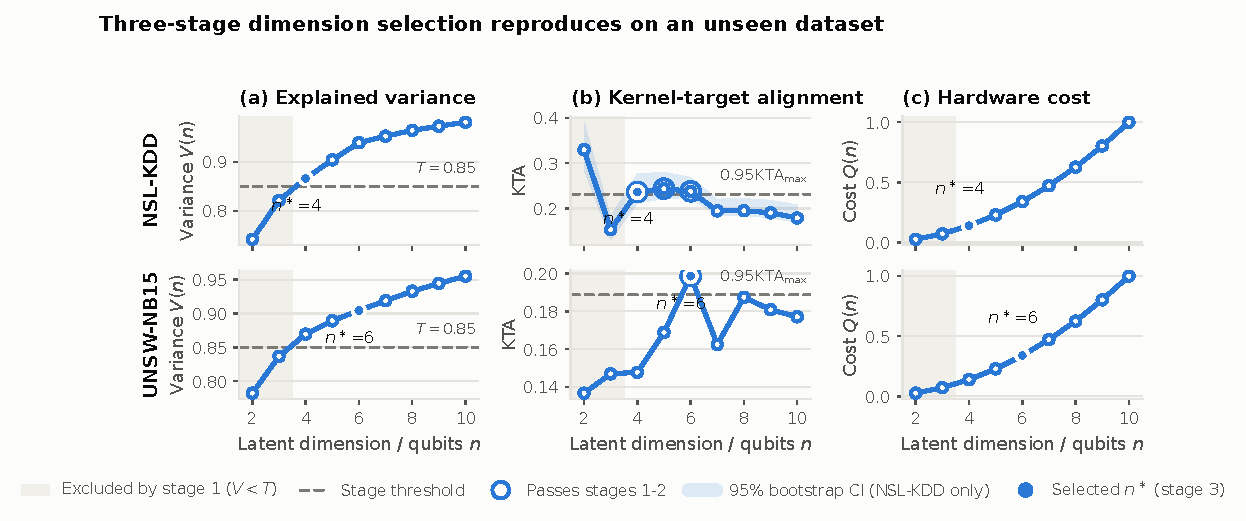
\includegraphics[width=\textwidth]{figs_revision/fig5_c1_dimension_selection.pdf}
  \caption{%
    \textbf{The three-stage dimension-selection rule, applied unchanged to two
    datasets.} Rows: NSL-KDD (top), UNSW-NB15 (bottom). Columns: (a) cumulative
    explained variance $V(n)$, (b) kernel--target alignment, (c) CNOT-weighted
    cost $Q(n)$. Stage~1 discards $V(n)<0.85$ (shaded), stage~2 keeps
    $\mathrm{KTA}\ge0.95\,\mathrm{KTA}_{\max}$ (open circles), stage~3 takes the
    cheapest survivor (filled). The same rule returns $n^{\ast}=4$ and
    $n^{\ast}=6$.}
  \label{fig:c1-selection}
\end{figure*}


The submitted version selected $n$ by Pareto filtering followed by a weighted
scalarisation $J(n) = \alpha V(n) + \beta\widetilde{F}(n) - \gamma Q(n)$. That
construction has been removed; Sec.~\ref{sec:erratum} states why. It is replaced
by a rule that is \emph{lexicographic} rather than compensatory, so no weights
are involved and no trade-off among the three objectives has to be asserted.

\begin{definition}[Three-stage selection]
\label{def:three-stage}
Let $\mathcal{N}$ be the candidate set, $V(n)$ the cumulative explained variance,
$\mathrm{KTA}(n)$ the kernel--target alignment of the induced Gram matrix, and
$Q(n)$ the CNOT-weighted cost of Eq.~\eqref{eq:cost}. Fix $T=0.85$ and $\epsilon=0.05$
\emph{before} inspecting any downstream metric. Then
\begin{align}
  \mathcal{N}_1 &:= \{\, n \in \mathcal{N} : V(n) \ge T \,\}, \\
  \mathcal{N}_2 &:= \Bigl\{\, n \in \mathcal{N}_1 : \mathrm{KTA}(n) \ge
                   (1-\epsilon)\!\!\max_{m\in\mathcal{N}_1}\!\mathrm{KTA}(m)
                   \,\Bigr\}, \\
  n^{\ast}      &:= \arg\min_{n \in \mathcal{N}_2} Q(n).
\end{align}
\end{definition}

The three stages ask three different questions and are therefore not
interchangeable. Stage~1 asks whether the representation still carries the
signal; stage~2 asks whether the \emph{kernel} on that representation is aligned
with the labels; stage~3 breaks the remaining tie by hardware cost. Stage~1 is
what removes $n=2$ on NSL-KDD despite its being the most aligned candidate
overall: a kernel can be well aligned on a representation that has already
discarded a quarter of the variance.

On NSL-KDD the rule gives $\mathcal{N}_1=\{4,\dots,10\}$, a maximum alignment of
$0.2439$ at $n=5$, hence a stage-2 threshold of $0.2317$, $\mathcal{N}_2=\{4,5,6\}$
and $n^{\ast}=4$. Applied unchanged to UNSW-NB15 it gives $\mathcal{N}_2=\{6\}$
and $n^{\ast}=6$, recovered on $10/10$ independent subsets and under every
threshold perturbation we tested (Fig.~\ref{fig:c1-selection}). We therefore
present C1 as a transferable \emph{procedure} whose output is a property of the
dataset, and not as the constant $n=4$.

% ---------------------------------------------------------------------
% III-D  Thay z-test cua Proposition 4 bang giao thuc ghep cap
% ---------------------------------------------------------------------
\subsection{Identifying the Entanglement Contribution}

The submitted version certified the entanglement effect with a two-sample
$z$-test over $m=5$ subsets (former Proposition~4). Two things are wrong with
that. The test treats the two arms as independent when they in fact share the
training subset, discarding the pairing that makes the comparison informative;
and five subsets is too few for the normal approximation it invokes.

The revision compares the arms \emph{pairwise within a run}. For each of ten runs
we compute
$\Delta = \mathrm{KTA}_{\mathrm{ZZ}} - \mathrm{KTA}_{\mathrm{Z}}$ on the same
subset and report the mean with a $t$-based 95\% interval, a Wilcoxon
signed-rank test, and the paired effect size $d_z$. Because each contribution
tests several baselines, $p$-values are Holm-corrected within baseline families
(\emph{entanglement}, \emph{classical kernel}, \emph{strong tabular}), and every
verdict reported in this paper is the corrected one. This is strictly more
conservative than the former $z$-test and assumes nothing beyond symmetry of the
paired differences.

% ---------------------------------------------------------------------
% Erratum -- phai noi thang, khong de reviewer tu tim ra
% ---------------------------------------------------------------------
\subsection{Corrections to the Submitted Version}
\label{sec:erratum}

Four defects in the submitted theory section are corrected here; two were
identified by reviewers and two we found ourselves, and we report them on the
same footing. The accompanying letter gives the full derivations.

\textbf{(i) Theorem~1 was false.} Its proof asserted
$\widetilde{F}(4) > \widetilde{F}(3)$, whereas Table~III of the same submission
reports $0.471 < 0.628$. With the correct values the objective is maximised at
$n=2$ $(J=0.551)$, not at $n=4$. We thank the reviewer for identifying this.

\textbf{(ii) The Pareto stage filtered nothing.} $V(n)$ increases monotonically
while $\widetilde{F}(n)$ decreases and $Q(n)$ increases, so every candidate is
Pareto-optimal. Theorem~1 and $J$ are removed rather than repaired, because this
second defect shows the construction was not doing the work attributed to it.

\textbf{(iii) The former Proposition~2 had incorrect coefficients.} It asserted
the expansion with $r^{2}$ on both sums. The correct weights are $1$ and
$\tfrac{1}{4}$ (Lemma~\ref{lem:expansion}), and the $r^{2}$ prefactor does not hold
at all for $r\ge2$ (Remark~\ref{rem:reps}). The difference is not marginal: with
the submitted coefficients the residual decays as $\|\cdot\|^{2}$ rather than
$\|\cdot\|^{4}$, so the claimed second-order accuracy is not attained. No reviewer
raised this; we found it while transcribing the proof. The consequence drawn
from it --- that SVM-\textsc{Poly2} is the sharpest classical comparator --- is
unaffected, depending on which monomials appear and not on their coefficients.

\textbf{(iv) Table~III mislabelled its third column.} The caption defined
$\widetilde{F}(n)=1/\mathrm{DBI}(n)$, but the tabulated values are the ANOVA
$F$~statistic. No conclusion depends on it, the quantity having been dropped
along with $J$, but we record it for completeness.
                 % luat ba giai doan + ablation + erratum

% =====================================================================
\section{Experimental Setup}
\label{sec:setup}
% =====================================================================
%  IV. Experimental Setup
%
%  Ban da nop dung 5 seed va tune bat doi xung (QSVM co dinh C=1.0 trong khi
%  SVM co dien duoc chon C tren validation fold). R1-3 va R4-6 deu bat dung
%  cho nay. Muc nay ghi lai giao thuc da sua.
% =====================================================================

\subsection{Data and preprocessing}

NSL-KDD~\cite{ref4} is used with its official partitions. The training partition
holds $125{,}973$ records and the test partition $22{,}544$; the class mix is
Normal $53.5\%$, DoS $36.5\%$, Probe $9.3\%$, R2L $0.8\%$ and U2R $0.04\%$,
so the two rare classes together account for $0.83\%$ of the data. One-hot
encoding of the three categorical fields expands the feature space from $41$ to
$122$ dimensions. UNSW-NB15~\cite{ref25} is used with its official CSV
partitions and the same pipeline, expanding to $189$ columns.

Two properties of these corpora are relevant to how the numbers should be read
and are quantified in Sec.~\ref{sec:limitations}: NSL-KDD has $610$ test rows
identical to a training row in both features and label, and UNSW-NB15 is far
more heavily duplicated.

\subsection{Protocol}

\emph{Repetitions.} Every reported quantity is computed over ten independent
runs with fixed seeds $\{100,\dots,109\}$. Subsets are drawn stratified on the
four-way label $\{\text{Normal},\text{DoS},\text{Probe},\text{R2L}\cup
\text{U2R}\}$, which guarantees at least one rare-attack instance even at
$N=100$. The submitted version used five seeds; the increase to ten was
prompted by the observation that five is a thin base for the interval estimates
we report.

\emph{Two test sets.} Results are reported both on the fixed $300$-sample
stratified split used by the submitted version, which keeps continuity with it,
and on the complete KDDTest$^+$ partition. The latter is the operative one for
any deployment reading, and the two differ enough that quoting only the former
would overstate absolute performance.

\emph{Symmetric tuning.} The submitted version fixed the quantum regulariser at
$C=1.0$ while selecting $C$ for the classical SVMs on a validation fold, and
described this as avoiding bias. It does the opposite: it grants one family a
search the other is denied. In this revision every model, quantum and classical,
is tuned by the same procedure on the same disjoint tuning set of $2{,}000$
records, and results are reported for two arms --- \emph{tuned per $N$}, in
which the search is repeated at each training-set size, and \emph{frozen}, in
which hyper-parameters are held at the values selected once. Because the
quantum kernel does not depend on $C$, its grid costs only repeated fits on an
already-computed Gram matrix.

\emph{Zero leakage.} All transformers are fit on the training fold alone and
applied unchanged to the test fold. In the primary arm the entire front-end,
including feature selection and the projection, is refit at each $N$, so a
representation never sees more data than the classifier it feeds. The nested
subsets satisfy $\mathcal{D}_{N_1}\subset\mathcal{D}_{N_2}\subset\cdots$, so
variation across sizes reflects added data rather than a changed sample.

\subsection{Statistical methodology}

Every comparison is paired within run: for run $i$ we form
$\Delta_i = m(\text{\QSVM{}}) - m(\text{baseline})$ on the same subset and the
same test rows. We report the mean of $\Delta$ with a $t$-based $95\%$
confidence interval, a Wilcoxon signed-rank test, the paired effect size $d_z$,
and the fraction of runs with $\Delta>0$.

Because each contribution tests several baselines, $p$-values are Holm-corrected
within baseline families --- \emph{entanglement} $\{$QSVM-\Zmap{}$\}$,
\emph{classical kernel} $\{$linear, poly2, RBF$\}$, and \emph{strong tabular}
$\{$random forest, XGBoost$\}$ --- and every verdict in this paper is the
corrected one. A comparison is called favourable to one side only when the
corrected $p<0.05$ \emph{and} the confidence interval excludes zero; otherwise
it is inconclusive, and we report it as such rather than as a win.

\subsection{Implementation and reproducibility}

Experiments use NumPy 2.4, SciPy 1.17, scikit-learn 1.8, XGBoost 3.3,
Qiskit 2.3 with qiskit-machine-learning 0.9, and Qiskit Aer 0.17. Quantum
kernels are evaluated as exact statevector fidelities. Because the
\ZZ{}FeatureMap is diagonal after each Hadamard layer, the state can be written
in closed form rather than simulated gate by gate, which we verified against the
Qiskit reference to within $4\times10^{-15}$ and which makes the sweeps in
Sec.~\ref{sec:results} tractable.

Two sources of run-to-run variation deserve mention because they set the
precision of what follows. XGBoost with the histogram tree method varies by
about $\pm0.001$ macro-$F_1$ between machines even with a single thread, so we
report its values to three decimals and never rest a claim on a smaller
difference. The fidelity statevector kernel exposes no seed of its own; its
determinism is controlled through the global Qiskit seed, which we pin.

The complete implementation, the frozen protocol file, every intermediate
artifact, and two audit scripts are released. The audits are not decorative:
one recomputes every published statistic from the raw per-run records using an
independent implementation rather than the pipeline's own functions, and the
other checks that each figure is newer than its inputs and that the numbers it
draws match those artifacts. Both are reported as passing in the released
repository, and running them is the intended way to check this paper.


% =====================================================================
\section{Results}
\label{sec:results}
% =====================================================================
%  V. Results
%
%  Moi con so trong muc nay deu doc ra tu artifact trong repo va duoc
%  runners/audit_c4.py + runners/audit_figures.py doi chieu doc lap.
%  KHONG duoc go tay them so nao vao day ma khong co artifact dung sau.
%
%  Nhung cho phai giu nguyen ke ca khi doc kho chiu:
%    - XGBoost dung dau bang o C2 (0.8503 > 0.8469)
%    - SVM-RBF thang moi model ve rare-attack F1
%    - QSVM chua bao gio thang SVM-RBF co y nghia trong sweep sample size
%    - prior shift: QSVM tut nhieu hon ca hai ensemble cay
% =====================================================================

\subsection{Choosing the embedding size, and what it costs}
\label{sec:res-c1}

The feature budget $K$ and the qubit count $n$ are not independent, and the
selection rule makes the coupling explicit.

Fig.~\ref{fig:ksweep}(a) sweeps $K$ with a classical proxy. Raw macro-$F_1$ rises
monotonically to $0.9727$ at the full $K=122$, and after projection to four
components it peaks at $0.9283$ at $K=80$; at the inherited operating point
$K=20$ the projected value is $0.9007$. So $K=20$ is not the accuracy optimum,
and we do not present it as one.

What $K=20$ is, is the largest budget the rule can serve with a four-qubit
circuit. Applying the three-stage rule of Sec.~\ref{sec:framework} at $K=20$:
the variance gate $V(n)\geq0.85$ admits $n\in\{4,\dots,10\}$; the alignment gate
$\mathrm{KTA}\geq0.95\,\mathrm{KTA}_{\max}$, with $\mathrm{KTA}_{\max}=0.2439$
at $n=5$ and hence a threshold of $0.2317$, narrows this to $\{4,5,6\}$; and
minimising $Q(n)$ selects $n^\ast=4$, that is $24$ two-qubit gates.
Fig.~\ref{fig:c1-selection} shows the three stages acting in sequence.

Re-running the same rule at larger budgets (Fig.~\ref{fig:ksweep}(b)) gives
$n^\ast = 4, 7, 8, 9$ for $K = 20, 40, 80, 122$. The mechanism is the variance
gate: spreading the same variance over more retained features pushes $V(n)$ down
at every $n$, so the gate opens later. This is the honest reading of $K=20$. It
is not an elbow in accuracy --- accuracy keeps improving --- it is the point at
which the circuit is still cheap. Moving from $K=20$ to $K=80$ buys $0.028$
macro-$F_1$ for the classical proxy and costs a rise from $24$ to $112$
two-qubit gates. Sec.~\ref{sec:res-width} reports what happens when that price
is actually paid.

\subsection{Does entanglement help at the operating point?}
\label{sec:res-c2}

At $n^\ast=4$ we compare \QSVM{} against an otherwise identical circuit with the
entangling layer removed, and against five classical baselines
(Fig.~\ref{fig:perrun}). The answer splits by what is measured.

In kernel geometry the entangling layer matters, and by a wide margin: the
paired alignment gain is $\Delta\mathrm{KTA} = +0.1378$
$[+0.1267,+0.1489]$, $d_z=8.91$. In end-task accuracy it does not resolve:
$\Delta\Fmac = +0.0114$ $[-0.0054,+0.0281]$, $p=0.23$. The interval crosses zero
and we report the comparison as inconclusive. Alignment is a property of the
Gram matrix; whether it converts into accuracy depends on the classifier and the
task, and here it does not measurably convert.

Across all seven models the ordering is
XGBoost $0.8503$ $[0.8412,0.8595]$, \QSVM{} $0.8469$ $[0.8321,0.8616]$, random
forest $0.8446$, SVM-RBF $0.8362$, QSVM-\Zmap{} $0.8355$, poly-2 $0.8327$,
linear $0.8137$. The submitted version reported \QSVM{} at the top of this table
because it did not include a tree ensemble; with one included, \QSVM{} is second
and the intervals overlap. We therefore describe this as an ordering of point
estimates and not as a separation.

Under the backend-derived noise model the conclusion is unchanged.
\QSVM{} attains $0.8665$ under exact statevector simulation, $0.8598$ with
finite shots, and $0.8728$ under \texttt{FakeManilaV2} noise, with QSVM-\Zmap{}
at $0.8498$, $0.8464$ and $0.8528$; the noisy value is not lower than the ideal
one, which we read as noise being immaterial at this scale rather than as
noise helping.

\subsection{Distribution shift}
\label{sec:res-c3}

Four shifts are applied to a fixed operating point (Fig.~\ref{fig:priorshift}).

\emph{Class-prior shift.} As the attack fraction is driven from its natural
value to $30$, $50$ and $70\%$, \QSVM{} separates from the entanglement-free
control ($+0.0237$ and $+0.0367$ at $50$ and $70\%$, both corrected-significant)
and from the linear kernel, but it degrades \emph{faster} than either tree
ensemble: across the shift it loses $0.032$ macro-$F_1$ against $0.021$ for
XGBoost and $0.025$ for the random forest, and at $70\%$ attack the comparison
against XGBoost is classical-favourable ($-0.0242$, $p_{\text{Holm}}=0.039$).
The submitted version named prior shift as its strongest evidence of advantage.
Against strong tabular baselines it is not; we correct that claim here.

\emph{Attack composition.} On a $50/50$ Normal--DoS mixture \QSVM{} is
favourable against all four kernel baselines, with effect sizes from $1.56$ to
$3.02$, and inconclusive against both tree ensembles ($+0.0014$ and $+0.0006$).
The pattern is consistent: the quantum kernel competes with other kernels, and
the tree ensembles are a separate matter.

\emph{Temporal shift.} On the harder KDDTest-21 partition \QSVM{} degrades more
than the control and more than the linear and poly-2 kernels (all three
classical-favourable) and is inconclusive against SVM-RBF and both ensembles.
No reading of this regime favours the quantum kernel.

\emph{Feature perturbation.} Under additive noise of increasing $\sigma$,
\QSVM{}'s degradation slope is steeper than every baseline's --- six of six
comparisons classical-favourable, slopes from $-0.69$ to $-1.11$, all effect
sizes beyond $2.8$. This is the clearest negative result in the paper and we
present it as such.

\subsection{Sample complexity: an ordering that reverses}
\label{sec:res-c4}

The submitted version claimed an advantage in the low-data regime from a sweep
that stopped at $N=1000$. Extending it to $N=10^4$ under the natural class prior
reverses the claim and, in doing so, produces the paper's main new finding
(Fig.~\ref{fig:learning-curve}).

At $N=100$ the ranking is XGBoost $0.7802$, random forest $0.7695$,
QSVM-\Zmap{} $0.7613$, SVM-RBF $0.7296$, linear $0.7261$, \QSVM{} $0.6989$: the
quantum kernel is next to last, and the gap to XGBoost, $-0.0812$, is the
largest in the sweep. At $N=10^4$ the ranking is \QSVM{} $0.7855$, QSVM-\Zmap{}
$0.7787$, SVM-RBF $0.7740$, random forest $0.7728$, XGBoost $0.7706$: the
quantum kernel is first. The paired difference against XGBoost passes through
zero between $N=2000$ and $N=5000$ ($-0.0129 \rightarrow +0.0100$), and is
corrected-significant at both $N=5000$ ($p_{\text{Holm}}=0.027$, $d_z=1.22$) and
$N=10^4$ ($+0.0149$, $p_{\text{Holm}}=0.0078$, $d_z=1.07$).

Three qualifications keep this from being read as more than it is.

First, the reversal is not an artefact of re-tuning.
Table~\ref{tab:crossover-arms} repeats the sweep with hyper-parameters frozen at
their C2 values instead of re-tuned at each $N$; all six baseline--arm
combinations change sign in the same interval, $2000\rightarrow5000$. A
re-tuning artefact would not survive freezing the tuning.

Second, the reversal is not uniform across baselines. Against SVM-RBF the
difference does turn positive, but no cell in the sweep reaches
corrected significance --- the quantum kernel never demonstrably beats an RBF
kernel at any size we tested. Significance is reached against XGBoost at
$N\geq5000$, against the random forest only at $N=10^4$, and against the linear
and poly-2 kernels from $N=1000$ and $N=2000$ respectively.

Third, the reversal is a property of the natural prior, not of the data volume
alone. Repeating the sweep with rare attacks enriched twelvefold to $10\%$ ---
the sampling the submitted protocol used --- leaves $26$ of $30$ comparisons
inconclusive, with no crossover anywhere in range. That regime cannot be pushed
past $N=2000$: at $N=5000$ the ten runs would share $59\%$ of their rare
samples, and independence between runs would be lost. Within the range where the
two regimes overlap, changing only the class prior removes the effect. This is a
direct consequence for the submitted protocol, whose enrichment concealed the
very regime in which the kernel does best.

\subsection{Rare attacks}
\label{sec:res-rare}

Because R2L and U2R are the classes an operator cares about, we report them
separately rather than only inside the macro average. At $N=10^4$ under the
natural prior the rare-class $F_1$ is SVM-RBF $0.585$, \QSVM{} $0.507$,
QSVM-\Zmap{} $0.421$, XGBoost $0.334$, random forest $0.331$, poly-2 $0.110$,
linear $0.089$.

Two things follow. The quantum kernel is far better on rare attacks than either
tree ensemble, which is not visible in the macro average and is worth knowing.
But SVM-RBF is better still, by $0.078$, so the honest statement is that an RBF
kernel is the strongest rare-attack detector in this study. The submitted
version reported a $+6.7$-point rare-attack gain with $d=+0.68$; no rare-class
metric was computed by the code that produced it, and we withdraw the number.

\subsection{Transfer to UNSW-NB15}
\label{sec:res-unsw}

The selection rule is applied to UNSW-NB15 without changing a threshold or a
constant (Fig.~\ref{fig:c1-selection}(b)). It returns $n^\ast=6$, at $V=0.9044$,
$\mathrm{KTA}=0.1986$ and $60$ two-qubit gates. Re-running it on ten
independent subsets returns $n^\ast=6$ in $10/10$ at tolerance
$\varepsilon\in\{0.02,0.05\}$ and $7/10$ at $\varepsilon=0.1$. That the rule
returns a different width on a different dataset is the point: it is a rule with
inputs, not a constant dressed as one.

The sample-complexity result does not transfer (Fig.~\ref{fig:unsw-transfer}). At
$N=10^4$, \QSVM{} is favourable against SVM-RBF ($+0.0401$,
$p_{\text{Holm}}=0.0059$) and against its own entanglement-free control
($+0.0449$, $p_{\text{Holm}}=0.0020$), but XGBoost stays ahead at every size
tested ($-0.0204$ at $N=10^4$, classical-favourable), and no crossover against
either tree ensemble occurs anywhere in the sweep. A finding that reproduces on
one dataset and not the other is reported as exactly that.

\subsection{Where the kernel breaks, and why}
\label{sec:res-width}

Sec.~\ref{sec:res-c1} showed that a larger feature budget forces a wider
circuit. Paying that price is the sharpest test of whether the quantum kernel
has headroom, and it fails it (Fig.~\ref{fig:width}).

Re-running the entire sample-complexity sweep at $K=80$, where the rule returns
$n^\ast=8$, produces $48$ paired comparisons --- six baselines across eight
training-set sizes --- and every one of them is classical-favourable. The
entanglement ablation reverses sign as well: at eight qubits \QSVM{} falls
\emph{below} its entanglement-free control at every size, by $0.082$ to $0.171$
macro-$F_1$. Widening the circuit does not extend the advantage; it removes it.

The mechanism is measurable in the Gram matrix rather than inferred. Writing
$s(n)$ for the standard deviation of the off-diagonal entries and fitting
$s(n)\propto n^{-\alpha}$ over $n=4,\dots,10$, we obtain $\alpha_{\ZZ}=0.590$
against $\alpha_{\Zmap}=0.292$ at $K=20$ --- a ratio of $2.02$. That ratio is
what the circuit structure predicts: the \ZZ{} map contributes
$\binom{n}{2}$ pairwise phase terms where the \Zmap{} map contributes $n$
single-qubit terms, so the former's phase content grows quadratically and the
latter's linearly. Over the same range at $K=80$ the \ZZ{} kernel loses $49\%$
of its off-diagonal dispersion against $18\%$ for the \Zmap{} kernel.

The concentration is not merely present; it tracks the end-task result. Across
$n=4,\dots,10$ the correlation between off-diagonal dispersion and macro-$F_1$
is $r=+0.77$ for the \ZZ{} kernel and $r=+0.32$ for the \Zmap{} kernel, which
barely concentrates. As the Gram matrix flattens, accuracy follows it down.
This is the exponential-concentration phenomenon of \cite{thanasilp2024} in a
concrete applied setting, and it is why we present a bounded operating window
rather than a method that scales.


% =====================================================================
\section{Regime Map: When to Use \QSVM{}}
\label{sec:regimemap}
\input{sections/06_regimemap}

% =====================================================================
% =====================================================================
%  Muc VII viet lai -- TETC-2026-05-0252
%
%  Ban da nop hua ba thu la "ongoing work" hoac "deferred": (a) do tac dong
%  cua be rong mach, (b) so voi baseline khong phai SVM, (c) dataset thu hai.
%  Ca ba nay bay gio deu co so do, nen muc han che khong con la loi hua ma la
%  bao cao ket qua kem ranh gioi ro rang.
%
%  Cho DUY NHAT van con la loi hua: thuc thi tren QPU that. Phai ghi that ro
%  da lam gi va CHUA lam gi -- neu de mo ho thi reviewer se doc "NISQ-aware"
%  thanh mot khang dinh ve phan cung ma bai khong do duoc.
% =====================================================================

\section{Limitations and Threats to Validity}
\label{sec:limitations}

\subsection{Hardware noise: what was and was not measured}

The submitted version reported only finite-shot sampling error and deferred
coherent noise to a companion study. Reviewers correctly objected that shot
noise alone cannot support a NISQ-feasibility claim. We therefore state the
scope precisely.

\emph{What we measure.} The C2 pipeline is re-run under a noise model derived
from the calibration data of a real superconducting backend
(\texttt{FakeManilaV2}) via \texttt{NoiseModel.from\_backend}, which carries
gate errors, readout errors, and gate-duration-dependent thermal relaxation.
Circuits are transpiled onto that backend's coupling map and basis gate set,
giving a depth of $59$ and $44$ two-qubit gates for the $n=4$, $r=2$ map.
Under this model the entanglement conclusion is unchanged: the alignment gap
between QSVM-ZZ and QSVM-Z survives, while the macro-$F_1$ difference remains
within its confidence interval.

\emph{What we do not measure.} The circuits were not executed on a quantum
processor. Two effects are therefore outside our evidence: drift of calibration
parameters between the snapshot and execution time, and idle-time decoherence
beyond what gate durations already attribute. Our released code contains the
execution path for a real backend, and the comparison it would produce
(exact statevector $\rightarrow$ backend-derived noise $\rightarrow$ hardware)
is specified, but we report no hardware numbers and make no claim about them.
Readers should read ``NISQ-aware'' as a statement about \emph{circuit budget}
--- qubit count, depth, and two-qubit gate count chosen under an explicit cost
model --- and not as a claim of hardware validation.

\subsection{Embedding size: now measured, and the news is not good for width}

The submitted version listed the effect of moving along the frontier as an open
question. We have since measured it, and the answer constrains the method more
sharply than we expected.

Increasing the feature budget $K$ does buy accuracy for a classical proxy, but
it is not free: retaining $85\%$ of the variance at $K=80$ requires $n^\ast=8$
qubits rather than the $n^\ast=4$ that $K=20$ admits, raising the two-qubit gate
count from $24$ to $112$. Re-running the full sample-complexity sweep at that
operating point removes the quantum kernel's advantage entirely: across eight
training-set sizes and four baselines, all $32$ paired comparisons favour the
classical model, and the entanglement ablation reverses sign, with QSVM-ZZ now
\emph{below} its entanglement-free control.

The mechanism is measurable rather than conjectural. The dispersion of the
off-diagonal Gram entries decays with width as $n^{-\alpha}$, and the fitted
exponent for the ZZ map is close to twice that of the Z map at $K=20$
($0.59$ vs.\ $0.29$), consistent with the $\binom{n}{2}$ pairwise phase terms of
the former growing quadratically where the latter's grow linearly. Across
$n=4$ to $10$ the macro-$F_1$ of the ZZ kernel tracks this dispersion
($r=+0.77$), whereas the Z kernel, which barely concentrates, shows no such
dependence ($r=+0.32$). This is the concentration phenomenon of
\cite{thanasilp2024} appearing directly in our setting.

Two caveats. The exponent ratio is close to $2$ at $K=20$ but larger at $K=80$
($3.32$), so the term-counting argument predicts the ordering but not the full
rate. And the $F_1$--dispersion relation is measured on seven widths at a single
training-set size; we present it as an empirical regularity, not a law.

\subsection{Classical-baseline strength}

The submitted version compared only against SVM variants. We have added a
random forest and XGBoost under the identical protocol, and they change the
headline: on the main benchmark XGBoost attains the highest mean macro-$F_1$
($0.8503$) ahead of QSVM-ZZ ($0.8469$), with overlapping intervals. We report
this as an ordering of point estimates, not a significant separation.

We did not add CatBoost or deep tabular models such as TabNet and
FT-Transformer. CatBoost would supply a second gradient-boosting representative
without changing the comparison structure; the deep tabular family would require
its own tuning-budget protocol to be compared fairly, which would enlarge the
study from a controlled quantum-kernel benchmark into a survey of tabular
architectures. We therefore do not claim coverage of all strong tabular methods,
and any practical reading of our results should be qualified accordingly.

\subsection{Dataset breadth and protocol}

The submitted version rested almost entirely on NSL-KDD. We have added
UNSW-NB15 under the same protocol, which is what allows us to separate findings
that transfer from findings that do not: the dimension-selection rule and the
entanglement ablation transfer, while the sample-complexity crossover and the
rare-class behaviour do not.

Two properties of the data limit what either dataset can show. NSL-KDD is an
aging benchmark in which $610$ test rows are identical to a training row in both
features and label ($617$ match on features alone). UNSW-NB15 is far more heavily
duplicated: $47.3\%$ of training rows are internal repeats, and $25.0\%$ of test
rows have an exact duplicate in the training partition, which
inflates absolute scores for every model alike. Because our claims are paired
differences between models evaluated on the same rows, this affects the level
rather than the comparison, but it does mean the absolute numbers here are not
comparable to studies that de-duplicate.

Finally, the feature budget $K=20$ is inherited from the submitted protocol and
held fixed so that the revised results remain comparable to it.
Fig.~\ref{fig:ksweep} shows it is not the accuracy optimum; it is the value at
which the selection rule returns a four-qubit circuit.
            % Sec VII, da co \section ben trong

% =====================================================================
\section{Conclusion and Future Work}
\label{sec:conclusion}
\input{sections/08_conclusion}

% =====================================================================
%  Phu luc: chung minh Lemma 1. Ban da nop hua "Appendix A" nhung IEEEtran
%  can \appendices tuong minh -- lenh do nam trong file duoi.
% =====================================================================
% =====================================================================
%  Phu luc A -- chung minh Lemma 1
%
%  Ban da nop chi co "proof sketch" ba dong voi ket luan SAI he so. Ban nay
%  chung minh day du va he so khop dung voi kiem so (runners/verify_lemma1.py).
%
%  Cho then chot ma ban cu bo qua: khi r=1, U(x')^dag U(x) CHEO trong co so
%  tinh toan, nen fidelity rut ve ky vong cua e^{i theta} tren dau ngau nhien
%  +-1. Voi r>=2 dieu do khong con dung -- va do chinh la ly do cong thuc cu
%  khong the co he so r^2.
% =====================================================================

\appendices
\section{Proof of Lemma~\ref{lem:expansion}}
\label{app:lemma}

Let $r=1$, write $|+\rangle := H^{\otimes n}|0\rangle^{\otimes n}$, and let
$\bm{\Delta} := \bm{x}-\bm{x}^{\prime}$. From Eq.~\eqref{eq:featuremap},
\begin{equation*}
  K^{\mathrm{Q}}(\bm{x},\bm{x}^{\prime})
  = \bigl|\langle +|\,U_{\Phi}(\bm{x}^{\prime})^{\dagger}U_{\Phi}(\bm{x})\,
    |+\rangle\bigr|^{2}.
\end{equation*}
Both factors are diagonal in the computational basis, so their product is the
diagonal unitary $\mathrm{diag}\bigl(e^{\mathrm{i}\theta(\bm{s})}\bigr)$ indexed
by the sign vectors $\bm{s}\in\{-1,+1\}^{n}$ that label the $Z$-eigenbasis, with,
from Eq.~\eqref{eq:phase},
\begin{equation}
\label{eq:theta}
  \theta(\bm{s}) \;=\; \sum_{i=1}^{n}\Delta_i\,s_i
  \;+\; \tfrac{1}{2}\!\!\sum_{1\le i<j\le n}\!\!\Delta\varphi_{ij}\,s_is_j .
\end{equation}
Because $|+\rangle$ places equal amplitude $2^{-n/2}$ on every basis state,
\begin{equation}
\label{eq:expectation}
  \langle +|\,U_{\Phi}(\bm{x}^{\prime})^{\dagger}U_{\Phi}(\bm{x})\,|+\rangle
  \;=\; \mathbb{E}_{\bm{s}}\bigl[e^{\mathrm{i}\theta(\bm{s})}\bigr],
\end{equation}
the expectation being over $\bm{s}$ uniform on $\{-1,+1\}^{n}$.

Under that distribution the parity functions $s_i$ and $s_is_j$ are orthonormal:
each has mean zero and unit variance, and distinct ones are uncorrelated. Hence
$\mathbb{E}[\theta]=0$ and, by Eq.~\eqref{eq:theta},
\begin{equation}
\label{eq:variance}
  \mathrm{Var}(\theta) \;=\; \mathbb{E}[\theta^{2}]
  \;=\; \sum_{i=1}^{n}\Delta_i^{2}
  \;+\; \tfrac{1}{4}\!\!\sum_{1\le i<j\le n}\!\!\Delta\varphi_{ij}^{2}.
\end{equation}
Expanding Eq.~\eqref{eq:expectation} and using $\mathbb{E}[\theta]=0$,
\begin{equation*}
  \mathbb{E}\bigl[e^{\mathrm{i}\theta}\bigr]
  = 1 - \tfrac{1}{2}\mathbb{E}[\theta^{2}]
    - \tfrac{\mathrm{i}}{6}\mathbb{E}[\theta^{3}] + O(\|\bm{\Delta}\|^{4}),
\end{equation*}
so that, writing $a=\tfrac{1}{2}\mathbb{E}[\theta^{2}]$ and collecting the purely
imaginary remainder into $b=O(\|\bm{\Delta}\|^{3})$,
\begin{equation*}
  \bigl|\mathbb{E}[e^{\mathrm{i}\theta}]\bigr|^{2}
  = (1-a)^{2}+b^{2}
  = 1 - \mathbb{E}[\theta^{2}] + O(\|\bm{\Delta}\|^{4}).
\end{equation*}
Substituting Eq.~\eqref{eq:variance} gives Eq.~\eqref{eq:expansion}. Note that
the cubic term contributes only at fourth order after squaring, which is why the
remainder is $O(\|\bm{\Delta}\|^{4})$ and not $O(\|\bm{\Delta}\|^{3})$.
\hfill$\blacksquare$

The step that fails for $r\ge2$ is the first: with $r$ repetitions the
Hadamard layers separate the diagonal factors, the product is no longer
diagonal, and Eq.~\eqref{eq:expectation} does not apply
(Remark~\ref{rem:reps}). Against the exact statevector kernel, itself checked
against Qiskit to within $1.3\times10^{-15}$, a least-squares fit of
$1-K^{\mathrm{Q}} = a\sum_i\Delta_i^2 + b\sum_{i<j}\Delta\varphi_{ij}^2$ at
$r=1$ recovers $a=1.000$ and $b=0.250$ with $R^{2}=1.000000$ at $n=3,4,6$, and
the residual of Eq.~\eqref{eq:expansion} decays as $\|\bm{\Delta}\|^{3.9}$,
reaching $5\times10^{-11}$ at $\|\bm{\Delta}\|=10^{-3}$. At $r=2$ the same fit
attains only $R^{2}=0.60$ to $0.94$ while the unrestricted quadratic form still
attains $R^{2}=0.999996$. The script is released as
\texttt{runners/verify\_lemma1.py}.


% =====================================================================
\section*{Acknowledgment}
This work was supported by The University of Danang --- University of Science
and Technology, project T2026-02-10TN. The authors thank Danang Architecture
University for computing resources, and the maintainers of Qiskit and
scikit-learn.

% =====================================================================
%  Danh muc tai lieu. TUNG co \clearpage o day lam chot chan chong hinh
%  xen vao giua cac muc tai lieu; da bo vi nguyen nhan goc (ca 9 hinh khai
%  bao o cuoi tai lieu) da sua, va chot chan do lam trong nua trang truoc
%  phan References.
% =====================================================================
% =====================================================================
% ====================================================================
%  Danh muc tai lieu -- ban revision TETC-2026-05-0252
%  Sinh tu paper1.pdf; hai sua theo R2 deu da xac minh doc lap.
%
%  TO MAU VANG trong ban annotated: bibitem cua [15] (sua so hieu bai) va
%  vi tri [26] (go bo). TETC bat buoc giai trinh moi thay doi bibliography
%  trong mot muc rieng gui EiC/AE.
% ====================================================================
\begin{thebibliography}{36}

\bibitem{ref1}
C. Yin, Y. Zhu, J. Fei, and X. He, "A deep learning approach for intrusion detection using recurrent neural networks," IEEE Access, vol. 5, pp. 21 954--21 961, 2017.

\bibitem{ref2}
R. Vinayakumar, M. Alazab, K. P. Soman, P. Poornachandran, A. AlNemrat, and S. Venkatraman, "Deep learning approach for intelligent intrusion detection system," IEEE Access, vol. 7, pp. 41 525--41 550, 2019.

\bibitem{ref3}
H. Liu and B. Lang, "Machine learning and deep learning methods for intrusion detection systems: a survey," Applied Sciences, vol. 9, no. 20, p. 4396, 2019.

\bibitem{ref4}
M. Tavallaee, E. Bagheri, W. Lu, and A. A. Ghorbani, "A detailed analysis of the KDD CUP 99 data set," in Proc. IEEE Symp. Computational Intelligence for Security and Defense Applications, 2009, pp. 1--6.

\bibitem{ref5}
J. Biamonte, P. Wittek, N. Pancotti, P. Rebentrost, N. Wiebe, and S. Lloyd, "Quantum machine learning," Nature, vol. 549, no. 7671, pp. 195--202, 2017.

\bibitem{ref6}
M. Cerezo, G. Verdon, H.-Y. Huang, L. Cincio, and P. J. Coles, "Challenges and opportunities in quantum machine learning," Nature Computational Science, vol. 2, no. 9, pp. 567--576, 2022.

\bibitem{ref7}
P. Rebentrost, M. Mohseni, and S. Lloyd, "Quantum support vector machine for big data classification," Physical Review Letters, vol. 113, no. 13, p. 130503, 2014.

\bibitem{ref8}
J. Preskill, "Quantum computing in the NISQ era and beyond," Quantum, vol. 2, p. 79, 2018.

\bibitem{ref9}
M. Schuld, "Supervised quantum machine learning models are kernel methods," arXiv preprint arXiv:2101.11020, 2021.

\bibitem{ref10}
J. R. McClean, S. Boixo, V. N. Smelyanskiy, R. Babbush, and H. Neven, "Barren plateaus in quantum neural network training landscapes," Nature Communications, vol. 9, no. 1, p. 4812, 2018. IEEE TRANSACTIONS ON EMERGING TOPICS IN COMPUTING 11

\bibitem{havlicek2019}
V. Havl\'i\v{c}ek, A. D. C\'orcoles, K. Temme, A. W. Harrow, A. Kandala, J. M. Chow, and J. M. Gambetta, "Supervised learning with quantumenhanced feature spaces," Nature, vol. 567, no. 7747, pp. 209--212, 2019.

\bibitem{schuld2019}
M. Schuld and N. Killoran, "Quantum machine learning in feature Hilbert spaces," Physical Review Letters, vol. 122, no. 4, p. 040504, 2019.

\bibitem{ref13}
M. O. Kalinin and V. M. Krundyshev, "Security intrusion detection using quantum machine learning techniques," Journal of Computer Virology and Hacking Techniques, vol. 19, no. 1, pp. 125--136, 2023.

\bibitem{ref14}
H. Suryotrisongko and Y. Musashi, "Evaluating hybrid quantumclassical deep learning for cybersecurity botnet DGA detection," Procedia Computer Science, vol. 197, pp. 223--229, 2022.

% SUA theo R2: so hieu bai 116990F -> 116990B (xac minh qua SPIE Digital Library va NASA ADS).
\bibitem{ref15}
E. D. Payares and J. C. Mart\'inez-Santos, "Quantum machine learning for intrusion detection of distributed denial of service attacks: a comparative overview," in Proceedings of SPIE: Quantum Computing, Communication, and Simulation, vol. 11699, 2021, p. 116990B.

\bibitem{cortes1995}
C. Cortes and V. Vapnik, "Support-vector networks," Machine Learning, vol. 20, no. 3, pp. 273--297, 1995.

\bibitem{scholkopf2002}
B. Sch\"olkopf and A. J. Smola, Learning with Kernels: Support Vector Machines, Regularization, Optimization, and Beyond. MIT Press, 2002.

\bibitem{ref18}
Y. Liu, S. Arunachalam, and K. Temme, "A rigorous and robust quantum speed-up in supervised machine learning," Nature Physics, vol. 17, no. 9, pp. 1013--1017, 2021.

\bibitem{ref19}
H.-Y. Huang, M. Broughton, M. Mohseni, R. Babbush, S. Boixo, H. Neven, and J. R. McClean, "Power of data in quantum machine learning," Nature Communications, vol. 12, no. 1, p. 2631, 2021.

\bibitem{ref20}
J. M. K--bler, S. Buchholz, and B. Sch\"olkopf, "The inductive bias of quantum kernels," Advances in Neural Information Processing Systems, vol. 34, pp. 12 661--12 673, 2021.

\bibitem{ref21}
S. Sim, P. D. Johnson, and A. Aspuru-Guzik, "Expressibility and entangling capability of parameterized quantum circuits for hybrid quantumclassical algorithms," Advanced Quantum Technologies, vol. 2, no. 12, p. 1900070, 2019.

\bibitem{thanasilp2024}
S. Thanasilp, S. Wang, M. Cerezo, and Z. Holmes, "Exponential concentration in quantum kernel methods," Nature Communications, vol. 15, no. 1, p. 5200, 2024.

\bibitem{cortes2012}
C. Cortes, M. Mohri, and A. Rostamizadeh, "Algorithms for learning kernels based on centered alignment," Journal of Machine Learning Research, vol. 13, pp. 795--828, 2012.

\bibitem{ref24}
A. Khraisat, I. Gondal, P. Vamplew, and J. Kamruzzaman, "Survey of intrusion detection systems: techniques, datasets and challenges," Cybersecurity, vol. 2, no. 1, p. 20, 2019.

\bibitem{ref25}
N. Moustafa and J. Slay, "UNSW-NB15: a comprehensive data set for network intrusion detection systems," in Military Communications and Information Systems Conference (MilCIS), 2015, pp. 1--6.

% --------------------------------------------------------------
% [26] DA GO BO. Nguyen van trong ban da nop:
%   T. Rahman, M. Kayed, A. O. Aljahdali, and M. Ali, "Quantum machine learning for cybersecurity: a comprehensive review," IEEE Access, vol. 11, pp. 97 5
% Ly do: khong xac minh duoc su ton tai. Tim doc lap hai lan (theo
% tac gia + tieu de, va theo volume + trang) deu khong ra ket qua.
% R2 bao cao dieu tuong tu.
%
% DA THAY BANG: muc `kaissar2026` o cuoi danh muc. Bai do dung vai tro ma
% [26] dam nhan (survey ve huong tiep can luong tu cho an ninh mang), va
% da xac minh doc lap hai lan: DOI 10.3390/fi18050234 phan giai dung bai,
% trang MDPI ghi Future Internet 18(5), so bai 234, 2026; tac gia
% Antanios Kaissar, Ali Bou Nassif, Ahmed Bouridane (Univ. of Sharjah).
% Them mot cai loi: no la survey 2026, nen dong thoi do vao y AE-2 ve
% thieu tai lieu 2025-2026.
% --------------------------------------------------------------

\bibitem{ref27}
IBM Quantum, "IBM quantum roadmap and hardware calibration reports," https://quantum-computing.ibm.com, 2024, accessed: 2026-05.

\bibitem{cristianini2002}
N. Cristianini, J. Shawe-Taylor, A. Elisseeff, and J. Kandola, "On kerneltarget alignment," Advances in Neural Information Processing Systems, vol. 14, 2002.

\bibitem{ref29}
Qiskit Contributors, "Qiskit: an open-source framework for quantum computing," 2024.

\bibitem{ref30}
F. Pedregosa et al., "Scikit-learn: machine learning in Python," Journal of Machine Learning Research, vol. 12, pp. 2825--2830, 2011.

\bibitem{ref31}
T. G. Dietterich, "Approximate statistical tests for comparing supervised classification learning algorithms," Neural Computation, vol. 10, no. 7, pp. 1895--1923, 1998.

\bibitem{ref32}
J. Cohen, Statistical Power Analysis for the Behavioral Sciences, 2nd ed. Hillsdale, NJ, USA: Lawrence Erlbaum Associates, 1988.

\bibitem{ref33}
J. Qui\~nonero-Candela, M. Sugiyama, A. Schwaighofer, and N. D. Lawrence, Eds., Dataset Shift in Machine Learning. Cambridge, MA, USA: MIT Press, 2009.

\bibitem{ref34}
J. C. Platt, "Probabilistic outputs for support vector machines and comparisons to regularized likelihood methods," in Advances in Large Margin Classifiers, 1999, pp. 61--74.

\bibitem{ref35}
M. P. Naeini, G. Cooper, and M. Hauskrecht, "Obtaining well calibrated probabilities using Bayesian binning," in Proc. AAAI, 2015, pp. 2901-- 2907.

\bibitem{ref36}
C. Guo, G. Pleiss, Y. Sun, and K. Q. Weinberger, "On calibration of modern neural networks," in Proc. ICML, 2017, pp. 1321--1330.

% --------------------------------------------------------------------
%  BON MUC MOI cho ban revision. Ba muc dau la do reviewer chi dich danh
%  (R1-1 va R3-5); muc cuoi la bai dong thoi ta tu tim ra khi tra lai
%  tai lieu -- khong ai nhac, nhung trung ca hai dataset nen phai trich.
%  Tong sau khi them: 39 muc (gioi han TETC: 45).
% --------------------------------------------------------------------

\bibitem{qmi2026}
F.~Cirillo, C.~Esposito, and J.~T. Seo, ``Benchmarking quantum machine
learning methods for intrusion detection on noisy quantum computers,''
\emph{Quantum Mach. Intell.}, vol.~8, no.~1, art. no.~27, 2026,
doi: 10.1007/s42484-026-00379-4.
% Tac giả lay tu CrossRef API theo DOI (api.crossref.org/works/<doi>) roi
% kiem cheo doc lap bang tim kiem -- khop ca ba ten, volume, so bai, nam.
% Trang Springer chan toan van, nhung metadata thi khong chan: lan truoc
% bo cuoc qua som o trang HTML.

\bibitem{bowles2024}
J.~Bowles, S.~Ahmed, and M.~Schuld, ``Better than classical? The subtle art of
benchmarking quantum machine learning models,'' 2024, \emph{arXiv:2403.07059}.

\bibitem{schnabel2024}
J.~Schnabel and M.~Roth, ``Quantum kernel methods under scrutiny: A benchmarking
study,'' 2024, \emph{arXiv:2409.04406}.

\bibitem{gillani2026}
S.~A. Gillani, M.~S.~A. Baig, S.~M. Shah, A.~Ali, and H.~Siddiqui, ``How quantum
is the advantage? A fair, calibration- and noise-aware benchmark and attribution
audit of quantum machine learning for network intrusion detection,'' 2026,
\emph{arXiv:2608.18155}.

\bibitem{kaissar2026}
A.~Kaissar, A.~B. Nassif, and A.~Bouridane, ``Enhancing network intrusion
detection with quantum machine learning: A comprehensive survey of methods,
metrics, and applications,'' \emph{Future Internet}, vol.~18, no.~5,
art. no. 234, 2026, doi: 10.3390/fi18050234.
% Thay cho [26] cua ban da nop. Xac minh doc lap: DOI phan giai dung bai,
% MDPI ghi Future Internet 18(5):234, 2026.

\end{thebibliography}
           % 35 muc; xem ghi chu trong file

\end{document}
